% ============================================================
% Chapter 24: Hilbert's Problem 23 — The Calculus of Variations
% ============================================================

\chapter{The Further Development of the Calculus of Variations}

\begin{partiallybox}
\textbf{Partially solved.} Hilbert's twenty-third and final problem called for the further development of the calculus of variations---a field that, by 1900, already had a rich history stretching back a century. Hilbert envisioned extending the direct method to more general problems and establishing rigorous foundations for the existence and regularity of minimizers. The response to this challenge has been extraordinary: the theory of the calculus of variations has grown into a vast edifice encompassing functional analysis, partial differential equations, geometric measure theory, and optimal control. Existence theorems are now available in remarkable generality (Tonelli, Morrey, De Giorgi), and the connection to PDE theory is deep and well understood. Yet fundamental questions remain open---regularity in the fully nonlinear case, the calculus of variations on manifolds, and the interplay between geometry and minimization continue to generate active research. The problem is best described as \emph{partially solved}: the foundations are secure, but the edifice is still growing.
\end{partiallybox}

% ------------------------------------------------------------
\section{Historical Context}
% ------------------------------------------------------------

The calculus of variations is one of the oldest branches of mathematical analysis, born from a question so natural that it seems to require no mathematics at all: \emph{what is the best way to do something?}

\begin{figure}[htbp]
\centering
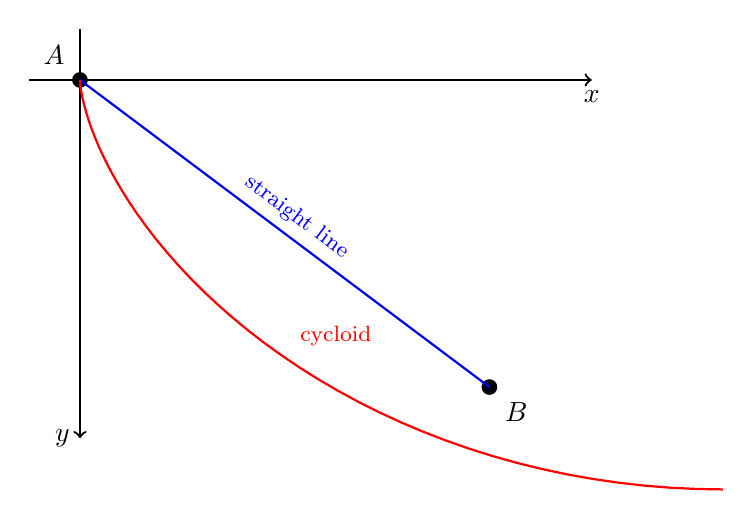
\begin{tikzpicture}[scale=1.3]
  \draw[thick,->] (-0.5,0) -- (5,0) node[below] {$x$};
  \draw[thick,->] (0,0.5) -- (0,-3.5) node[left] {$y$};
  \node[circle,fill,inner sep=2pt,label=above left:$A$] at (0,0) {};
  \node[circle,fill,inner sep=2pt,label=below right:$B$] at (4,-3) {};
  \draw[thick,blue] (0,0) -- (4,-3)
    node[midway,above,sloped] {\footnotesize straight line};
  \draw[thick,red,domain=0:pi,samples=50,variable=\t]
    plot ({2*(\t - sin(\t r))},{2*(cos(\t r) - 1)});
  \node[red] at (2.5,-2.5) {\footnotesize cycloid};
\end{tikzpicture}
\caption{The brachistochrone problem: a bead slides from $A$ to $B$ under gravity. The straight (Euclidean) path (blue) is the shortest distance, but the cycloid (red) gives the shortest time of descent.}
\label{fig:brachistochrone}
\end{figure}

\subsection{The Brachistochrone Problem}

The story begins in 1696, when Johann Bernoulli posed a challenge to the mathematicians of Europe. A bead slides without friction along a wire connecting two points $A$ and $B$, where $B$ is lower than $A$. Under the influence of gravity alone, along what shaped wire does the bead travel from $A$ to $B$ in the \emph{shortest time}?

This is the \textbf{brachistochrone problem} (from the Greek \emph{brachistos}, ``shortest,'' and \emph{chronos}, ``time''). The answer is not a straight line---that would be the shortest \emph{distance}, but not the fastest \emph{path}. The bead gains speed as it descends, so a path that dips steeply at the start and then levels out can be faster than the direct route.

The solution, found independently by Newton, Leibniz, L'H\^opital, and the Bernoulli brothers, is a \textbf{cycloid}---the curve traced by a point on the rim of a rolling wheel. If $A$ is at the origin and $B$ is at $(x_1, y_1)$ with $y_1 < 0$ (taking the $y$-axis pointing downward), the cycloid is parametrized by
\[
    x = R(\theta - \sin\theta), \qquad y = R(1 - \cos\theta),
\]
where $R$ is chosen so that the curve passes through $B$.

The brachistochrone problem is a \textbf{variational problem}: we seek a function (the shape of the wire) that minimizes a quantity (the travel time) that depends on the function and its derivative. Specifically, the time of descent along a curve $y = y(x)$ from $A = (0,0)$ to $B = (x_1, y_1)$ is
\[
    T[y] = \int_0^{x_1} \frac{\sqrt{1 + (y')^2}}{\sqrt{2gy}} \, dx.
\]
The brachistochrone is the curve $y(x)$ that minimizes this integral among all smooth curves connecting $A$ to $B$.

\subsection{Euler and Lagrange: The Founding of the Calculus of Variations}

The brachistochrone was a special case of a much more general question. In 1744, Leonhard Euler published his \emph{Methodus inveniendi lineas curvas}, which laid the foundations of the calculus of variations. Euler asked: given a functional of the form
\[
    J[y] = \int_a^b F(x, y(x), y'(x)) \, dx,
\]
what differential equation must $y$ satisfy to be an extremum?

Euler's answer, refined and generalized by Joseph-Louis Lagrange in 1755, is the \textbf{Euler--Lagrange equation}:
\[
    \frac{\partial F}{\partial y} - \frac{d}{dx}\frac{\partial F}{\partial y'} = 0.
\]
This is a second-order ordinary differential equation. Any smooth extremum of $J[y]$ must satisfy it---just as a differentiable extremum of a function of several variables must have vanishing partial derivatives.

\begin{theorem}[Euler--Lagrange Equation]
\label{thm:euler-lagrange}
Let $F = F(x, y, y')$ be a $C^2$ function, and let $y \in C^2([a,b])$ be a function with $y(a) = A$, $y(b) = B$ that minimizes (or maximizes) the functional
\[
    J[y] = \int_a^b F(x, y(x), y'(x)) \, dx
\]
among all such functions. Then $y$ satisfies the Euler--Lagrange equation
\[
    F_y(x, y, y') - \frac{d}{dx} F_{y'}(x, y, y') = 0
\]
on the interval $[a, b]$.
\end{theorem}

\begin{proof}
Suppose $y$ is a minimizer. For any smooth function $\eta$ with $\eta(a) = \eta(b) = 0$, consider the perturbed function $y + \varepsilon \eta$. Define
\[
    \phi(\varepsilon) = J[y + \varepsilon \eta] = \int_a^b F(x, y + \varepsilon \eta, y' + \varepsilon \eta') \, dx.
\]
Since $y$ minimizes $J$, we have $\phi'(0) = 0$. Computing the derivative under the integral sign:
\[
    \phi'(0) = \int_a^b \left[ F_y(x, y, y') \eta + F_{y'}(x, y, y') \eta' \right] dx = 0.
\]
Integrating the second term by parts:
\[
    \int_a^b F_{y'} \eta' \, dx = \left[ F_{y'} \eta \right]_a^b - \int_a^b \frac{d}{dx} F_{y'} \cdot \eta \, dx = -\int_a^b \frac{d}{dx} F_{y'} \cdot \eta \, dx,
\]
since $\eta(a) = \eta(b) = 0$. Therefore,
\[
    \int_a^b \left[ F_y - \frac{d}{dx} F_{y'} \right] \eta \, dx = 0.
\]
Since this holds for all admissible $\eta$, the fundamental lemma of the calculus of variations implies $F_y - \frac{d}{dx} F_{y'} = 0$ on $[a,b]$.
\end{proof}

Lagrange's great innovation was not just the equation itself, but the \emph{method}: he introduced the idea of varying the function $y$ by an infinitesimal amount and requiring the first-order change in $J$ to vanish. This is the prototype of all variational arguments, and it connects directly to the idea of a \emph{directional derivative} in infinite-dimensional spaces---a connection that would not be made precise until the twentieth century.

\subsection{Weierstrass and the Rigorization}

By the late nineteenth century, the calculus of variations had produced many beautiful results, but its foundations were shaky. Euler and Lagrange had derived necessary conditions for extrema (the Euler--Lagrange equation), but the \emph{sufficiency}---the conditions under which a solution to the Euler--Lagrange equation actually minimizes the functional---was not understood.

Karl Weierstrass, in his lectures at Berlin in the 1870s, put the subject on a rigorous footing. He introduced the concept of a \textbf{strong minimum} versus a \textbf{weak minimum}, and he gave a necessary condition (the \textbf{Weierstrass $E$-function}) that a minimizer must satisfy. He also constructed counterexamples showing that solutions to the Euler--Lagrange equation need not be minimizers without additional hypotheses.

But Weierstrass also identified a deeper problem: \emph{does a minimizer exist at all?} Given a functional $J[y]$, is there always a function $y$ that achieves the infimum? Weierstrass's own work on the Dirichlet principle (which we discussed in Chapter~\ref{ch:problem-20}) showed that the answer can be no: one can have a sequence of functions with $J[y_n] \to \inf J$, but no function $y$ with $J[y] = \inf J$. The infimum is not always a minimum.

This is the central problem that Hilbert's twenty-third problem addresses: \emph{under what conditions does a minimizer exist, and how can we prove existence directly?}

\subsection{The Direct Method}

Hilbert's approach, which we also encountered in Chapter~\ref{ch:problem-20}, was to work not in the space of smooth functions but in a larger, complete space where minimizing sequences are forced to have convergent subsequences. This is the \textbf{direct method in the calculus of variations}:

\begin{enumerate}
    \item \textbf{Bounded below:} Show that the functional $J[y]$ is bounded from below on the admissible class.
    \item \textbf{Minimizing sequence:} Take a sequence $\{y_n\}$ with $J[y_n] \to \inf J$.
    \item \textbf{Compactness:} Extract a convergent subsequence (in an appropriate topology) with limit $y$.
    \item \textbf{Lower semicontinuity:} Show that $J[y] \leq \liminf J[y_n]$, so $y$ is a minimizer.
\end{enumerate}

The difficulty lies in steps 3 and 4: one needs the right notion of convergence, and one needs the functional to be lower semicontinuous with respect to that convergence. Hilbert's insight was that \emph{weak convergence} in a Hilbert space---convergence that preserves inner products but not norms---provides the right framework. The functional $J[y]$, when it is convex and coercive, is weakly lower semicontinuous, and bounded sequences in Hilbert spaces have weakly convergent subsequences (by the Banach--Alaoglu theorem).

% ------------------------------------------------------------
\section{The Problem}
% ------------------------------------------------------------

\begin{problem_statement}[Hilbert's Twenty-Third Problem]
Develop the calculus of variations into a rigorous and general theory. In particular, extend the direct method to a wide class of variational problems, study the existence and regularity of minimizers, and investigate the relationship between variational principles and differential equations.
\end{problem_statement}

Hilbert's problem is deliberately open-ended. It does not ask for a single theorem but for the \emph{development of a theory}---one that would place the calculus of variations on the same rigorous footing as other branches of analysis. The key questions include:

\begin{enumerate}
    \item \textbf{Existence:} Given a functional $J$, does a minimizer exist? Under what conditions on $F$, the domain, and the boundary data?
    \item \textbf{Regularity:} If a minimizer exists, how smooth is it? Is it $C^2$? Analytic? Does it depend on the smoothness of $F$?
    \item \textbf{Higher dimensions:} The classical calculus of variations deals with functionals involving functions of one variable. How does the theory extend to functions of several variables, where the Euler--Lagrange equation becomes a PDE?
    \item \textbf{Constraints and boundary conditions:} How does the theory handle integral constraints (isoperimetric problems), inequality constraints, and various types of boundary conditions?
\end{enumerate}

% ------------------------------------------------------------
\section{Key Developments}
% ------------------------------------------------------------

\subsection{Tonelli's Existence Theorem (1910s--1920s)}

The first systematic answer to the existence question came from Leonida Tonelli, who developed the direct method into a powerful and general tool over the course of two decades, culminating in his magisterial \emph{Theorie der Funktionen} (1921--1923).

Tonelli's key contribution was to identify the right class of functionals for which the direct method works. A functional of the form
\[
    J[y] = \int_\Omega F(x, y(x), \nabla y(x)) \, dx
\]
admits a minimizer if:
\begin{enumerate}
    \item $F$ is \textbf{convex} in the gradient variable $p = \nabla y$.
    \item $F$ satisfies a \textbf{coercivity} condition: $F(x, y, p) \to \infty$ as $|p| \to \infty$.
    \item The admissible functions satisfy appropriate boundary conditions and lie in a suitable Sobolev space.
\end{enumerate}

\begin{theorem}[Tonelli's Existence Theorem]
\label{thm:tonelli}
Let $\Omega \subset \mathbb{R}^n$ be a bounded domain with Lipschitz boundary, and let $F: \Omega \times \mathbb{R} \times \mathbb{R}^n \to \mathbb{R}$ be a function satisfying:
\begin{enumerate}
    \item $F$ is measurable in $x$ and continuous in $(y, p)$;
    \item $F$ is convex in $p$ for each $(x, y)$;
    \item There exist constants $c_0 > 0$ and $c_1 \geq 0$ such that $F(x, y, p) \geq c_0 |p|^2 - c_1$ for all $(x, y, p)$.
\end{enumerate}
Let $g \in H^1(\Omega)$ be given boundary data. Then the functional
\[
    J[u] = \int_\Omega F(x, u(x), \nabla u(x)) \, dx
\]
attains its minimum on the set $\{u \in H^1(\Omega) : u - g \in H^1_0(\Omega)\}$. That is, there exists a minimizer $u \in H^1(\Omega)$ with $J[u] = \inf J$.
\end{theorem}

The proof is a direct application of the direct method. The coercivity condition ensures that minimizing sequences are bounded in $H^1(\Omega)$. Since $H^1(\Omega)$ is a reflexive Banach space (it is a Hilbert space), the Banach--Alaoglu theorem provides a weakly convergent subsequence. The convexity of $F$ in $p$ ensures that $J$ is weakly lower semicontinuous---the key technical ingredient. The infimum is therefore attained.

Tonelli's theorem is the cornerstone of the modern calculus of variations. Its hypotheses are general enough to cover most problems arising in physics and geometry, and its conclusion is as strong as one could hope: a minimizer exists.

\subsection{The Connection to Functional Analysis}

The direct method reveals a deep connection between the calculus of variations and \textbf{functional analysis}---the study of infinite-dimensional vector spaces with topological structure.

The key spaces are:

\begin{definition}[Hilbert space]
A \textbf{Hilbert space} $H$ is a complete inner product space. The prototype is $\ell^2$, the space of square-summable sequences, and its continuous analogue $L^2(\Omega)$, the space of square-integrable functions.
\end{definition}

\begin{definition}[Sobolev space]
The \textbf{Sobolev space} $H^1(\Omega)$ consists of functions $u \in L^2(\Omega)$ whose weak first derivatives also lie in $L^2(\Omega)$, equipped with the inner product
\[
    \langle u, v \rangle_{H^1} = \int_\Omega \left( uv + \nabla u \cdot \nabla v \right) dx.
\]
\end{definition}

The direct method works because of three fundamental facts:

\begin{enumerate}
    \item \textbf{Weak compactness:} Bounded sets in a reflexive Banach space are weakly precompact (Banach--Alaoglu). This provides the convergent subsequence.
    \item \textbf{Weak lower semicontinuity:} If $J$ is convex and continuous, then $J$ is weakly lower semicontinuous: $u_n \rightharpoonup u$ weakly implies $J[u] \leq \liminf J[u_n]$. This ensures the limit is a minimizer.
    \item \textbf{Coercivity:} If $J[u] \to \infty$ as $\|u\| \to \infty$, then minimizing sequences are bounded, and weak compactness applies.
\end{enumerate}

These ideas, developed by Hilbert, Banach, Fr\'echet, and others in the early twentieth century, transformed the calculus of variations from an ad hoc collection of techniques into a systematic theory. The language of functional analysis---weak convergence, reflexivity, Sobolev spaces---is now the natural setting for variational problems.

\subsection{Higher-Order Variational Problems and PDEs}

When the unknown is a function of several variables, say $u: \Omega \subset \mathbb{R}^n \to \mathbb{R}$, the Euler--Lagrange equation becomes a \textbf{partial differential equation}. For the functional
\[
    J[u] = \int_\Omega F(x, u(x), \nabla u(x)) \, dx,
\]
the Euler--Lagrange equation is
\[
    F_u - \sum_{i=1}^n \frac{\partial}{\partial x_i} F_{p_i}(x, u, \nabla u) = 0,
\]
where $p_i = \partial u / \partial x_i$. This is a second-order PDE. For example, if $F(x, y, p) = \frac{1}{2}|p|^2$, the Euler--Lagrange equation is $\Delta u = 0$---Laplace's equation.

The connection between variational problems and PDEs is bidirectional:
\begin{itemize}
    \item Given a variational problem, the Euler--Lagrange equation provides a PDE that the minimizer must satisfy.
    \item Given a PDE, one can often construct a functional whose minimizer is a solution to the PDE.
\end{itemize}

This duality is one of the most powerful ideas in mathematical analysis. It means that existence theorems for PDEs can be proved by variational methods (finding minimizers), and regularity theorems for minimizers can be proved by PDE techniques (bootstrap arguments, Schauder estimates).

\subsection{Regularity Theory}

A natural question arises: if $u \in H^1(\Omega)$ minimizes $J[u]$ and $F$ is smooth, how smooth is $u$?

For \textbf{quadratic} functionals (where $F$ is a quadratic form in $p$), the Euler--Lagrange equation is linear, and elliptic regularity theory (Chapter~\ref{ch:problem-19}) shows that $u$ is as smooth as the data permits: $u \in C^\infty(\Omega)$ if $F$ and $\Omega$ are smooth, and in fact $u$ is real-analytic.

For \textbf{nonlinear} functionals, regularity is more subtle. The fundamental result is:

\begin{theorem}[Interior Regularity for Minimizers]
Let $u \in H^1(\Omega)$ minimize $J[u]$ where $F$ is $C^2$ and uniformly convex in $p$. Then $u \in C^{1,\alpha}_{\mathrm{loc}}(\Omega)$ for some $\alpha \in (0,1)$---that is, $u$ has locally H\"older-continuous first derivatives.
\end{theorem}

This is a deep result, proved in stages by De Giorgi (1957), Nash (1958), and Morrey (1968). The regularity is in general \emph{not} better than $C^{1,\alpha}$: there are examples of minimizers that are not $C^2$. This stands in stark contrast to the linear case, where analyticity is the norm.

\subsection{Optimal Control Theory}

In the mid-twentieth century, the calculus of variations underwent a dramatic transformation through its connection to \textbf{optimal control theory}---the mathematical theory of how to steer a dynamical system to achieve a desired outcome at minimum cost.

The key figure is Lev Pontryagin, who in 1956 formulated the \textbf{Pontryagin maximum principle}, a necessary condition for optimality in control problems that generalizes the Euler--Lagrange equation. The basic problem of optimal control is:

\begin{problem_statement}[Optimal Control]
Given a dynamical system $\dot{x} = f(x, u)$ with state $x(t)$ and control $u(t)$, and a cost functional
\[
    J[u] = \int_0^T L(x(t), u(t)) \, dt + \Phi(x(T)),
\]
find the control $u$ that minimizes $J$ subject to the dynamics and boundary conditions.
\end{problem_statement}

Pontryagin's principle states that an optimal control $u^*$ must satisfy:
\[
    H(x^*(t), u^*(t), \lambda(t)) = \max_{u \in \mathcal{U}} H(x^*(t), u, \lambda(t)),
\]
where $H(x, u, \lambda) = \lambda \cdot f(x, u) - L(x, u)$ is the \textbf{Hamiltonian} and $\lambda(t)$ is the \textbf{costate} (or adjoint) variable satisfying an adjoint differential equation. This is the variational principle reformulated for problems with constraints on the control variable---constraints that arise naturally in engineering applications.

The connection to the classical calculus of variations is direct: when there are no constraints on the control and $f(x, u) = u$, the Pontryagin maximum principle reduces to the Euler--Lagrange equation. But optimal control extends the variational framework to handle inequality constraints, switching costs, and discontinuous controls---problems that arise in aerospace engineering, robotics, economics, and biology.

\subsection{Modern Applications}

The calculus of variations, far from being a historical artifact, is at the heart of much of modern mathematics and science.

\paragraph{Minimal surfaces.}
A \textbf{minimal surface} is a surface that minimizes area among all surfaces with a given boundary. The classical \textbf{Plateau problem}---given a wire frame in space, does a soap film spanning it exist?---is a variational problem. It was solved by Jesse Douglas and Richard Courant independently in 1930 (Douglas received the Fields Medal for this work). The modern theory uses geometric measure theory and the space of functions of bounded variation (BV spaces) to handle surfaces that may have singularities.

\paragraph{Geometric flows.}
The \textbf{Ricci flow}, introduced by Richard Hamilton in 1982, is a variational evolution equation for Riemannian metrics. It was the key ingredient in Grigori Perelman's proof of the Poincar\'e conjecture (2002--2003). The \textbf{mean curvature flow} is the gradient flow of the area functional and is used to study the structure of submanifolds.

\paragraph{Materials science.}
The equilibrium configuration of a crystalline solid is determined by minimizing a free energy functional that includes elastic, surface, and interaction terms. The \textbf{phase-field models} of materials science are gradient flows of such functionals, and their analysis relies on the direct method and its refinements.

\paragraph{General relativity.}
Einstein's field equations can be derived from the \textbf{Einstein--Hilbert action}, a variational principle for the metric tensor of spacetime. The search for solutions---black holes, gravitational waves, cosmological models---is fundamentally a variational problem.

% ------------------------------------------------------------
\section{Current Status: Partially Solved}
% ------------------------------------------------------------

\begin{partiallybox}
Hilbert's twenty-third problem is \textbf{partially solved} in the following sense. The foundations of the calculus of variations are secure: Tonelli's existence theorem provides minimizers for a wide class of problems, the direct method is a powerful and flexible tool, and the connection to functional analysis and PDE theory is deep and well understood. Regularity theory for minimizers of convex functionals is well developed (De Giorgi--Nash--Morrey), and optimal control theory has extended the variational framework to problems with constraints and discontinuities.

However, major questions remain open:
\begin{itemize}
    \item \textbf{Regularity for non-convex problems:} For functionals that are not convex in the gradient, minimizers may have singularities, and the regularity theory is far from complete.
    \item \textbf{The calculus of variations on manifolds:} Minimizing functionals defined on spaces of maps between Riemannian manifolds (harmonic maps, minimal immersions) presents fundamental difficulties related to the topology of the target space.
    \item \textbf{Stochastic variational problems:} Variational principles involving randomness (stochastic differential games, mean-field games) are a rapidly growing area.
    \item \textbf{Computational methods:} While the finite element method is mature, the numerical analysis of variational problems with singularities, free boundaries, and high-dimensional parameter spaces remains challenging.
\end{itemize}

The spirit of Hilbert's challenge---to develop the calculus of variations into a complete and rigorous theory---has been largely fulfilled, but the subject continues to evolve and to surprise.
\end{partiallybox}

% ------------------------------------------------------------
\section*{Common Questions}
% ------------------------------------------------------------

\begin{description}[font=\bfseries, leftmargin=2em, style=nextline]

\item[Q: What's the difference between calculus of variations and ordinary calculus?]\hfill\\
Ordinary calculus finds the $x$ that minimizes a function $f(x)$---a finite-dimensional problem. The calculus of variations finds the \emph{function} $y(x)$ that minimizes a functional $J[y]$---an infinite-dimensional problem. Instead of setting a derivative to zero, you set the first variation (directional derivative with respect to a perturbation) to zero, which yields the Euler--Lagrange equation.

\item[Q: What is the Euler--Lagrange equation and why is it so important?]\hfill\\
It is the necessary condition $F_y - \frac{d}{dx}F_{y'} = 0$ that any smooth minimizer of $J[y] = \int F(x,y,y')\,dx$ must satisfy. It transforms a variational problem into a differential equation, bridging the calculus of variations and PDE theory. Almost every law of physics---from Newton's laws to Einstein's field equations---can be derived from a variational principle whose Euler--Lagrange equation is the governing equation.

\item[Q: What is the brachistochrone problem and why is it famous?]\hfill\\
It asks for the shape of a wire along which a bead slides fastest under gravity (shortest time, not shortest distance). The answer is a cycloid. It is famous because it launched the calculus of variations in 1696, drew contributions from Newton, Leibniz, and the Bernoullis, and showed that the fastest path is not the obvious straight line---a counterintuitive result that epitomizes variational thinking.

\item[Q: What is the direct method?]\hfill\\
The direct method proves existence of a minimizer without solving the Euler--Lagrange equation: (1) take a minimizing sequence, (2) extract a convergent subsequence using weak compactness in a Sobolev space, (3) show the functional is lower semicontinuous so the limit is a minimizer. It turns an analytic existence problem into a topological compactness argument.

\item[Q: Why is convexity needed for existence?]\hfill\\
If $F$ is convex in $p = y'$, the functional $J$ is weakly lower semicontinuous---a limit of a minimizing sequence cannot have larger energy than the sequence. Without convexity, the functional may ``see'' fine oscillations that blow up in the limit, and the infimum may not be attained. Convexity ensures that averaging lowers the energy.

\item[Q: How does the calculus of variations connect to optimal control?]\hfill\\
Optimal control generalizes the calculus of variations by allowing constraints on the derivative (control variables may be bounded, dynamics may be nonlinear). Pontryagin's maximum principle plays the role of the Euler--Lagrange equation. The modern theory of optimal control is essentially the calculus of variations with inequality constraints, and it is the mathematical foundation of robotics, aerospace engineering, and economics.

\end{description}

% ------------------------------------------------------------
\section*{Exercises}
% ------------------------------------------------------------

\begin{enumerate}

    \item \textbf{The Euler--Lagrange equation for specific functionals.}
    Derive the Euler--Lagrange equation for each of the following functionals, and identify the resulting differential equation:
    \begin{enumerate}
        \item $J[y] = \int_0^1 \left[(y')^2 + y^2\right] dx$ (the quadratic functional).
        \item $J[y] = \int_0^1 \sqrt{1 + (y')^2} \, dx$ (the arc length functional).
        \item $J[y] = \int_0^\pi \left[(y')^2 - y^2\right] dx$.
        \item $J[y] = \int_1^e \frac{(y')^2}{x} \, dx$ with $y(1) = 0$, $y(e) = 1$.
    \end{enumerate}

    \item \textbf{The brachistochrone.}
    \begin{enumerate}
        \item Starting from the time-of-descent functional
        \[
            T[y] = \int_0^{x_1} \frac{\sqrt{1 + (y')^2}}{\sqrt{2gy}} \, dx,
        \]
        derive the Euler--Lagrange equation. (Hint: since the integrand $F$ does not depend explicitly on $x$, you can use the \textbf{Beltrami identity}: $F - y' F_{y'} = \text{constant}$.)
        \item Show that the cycloid $x = R(\theta - \sin\theta)$, $y = R(1 - \cos\theta)$ satisfies this equation.
        \item Explain physically why the cycloid is faster than a straight line.
    \end{enumerate}

    \item \textbf{Geodesics.}
    \begin{enumerate}
        \item Write the arc length functional for a curve on a surface $S$ parametrized by $(u, v) \mapsto \mathbf{r}(u, v)$:
        \[
            L[\gamma] = \int_a^b \sqrt{E \dot{u}^2 + 2F \dot{u}\dot{v} + G \dot{v}^2} \, dt
        \]
        where $E, F, G$ are the coefficients of the first fundamental form.
        \item Show that geodesics (minimizers of $L$) satisfy the geodesic equations, which are second-order ODEs involving the Christoffel symbols.
        \item Verify that geodesics on the plane $\mathbb{R}^2$ (with $E = G = 1$, $F = 0$) are straight lines.
    \end{enumerate}

    \item \textbf{The isoperimetric problem.}
    The classical isoperimetric problem asks: among all closed curves of fixed length $\ell$, which one encloses the greatest area?
    \begin{enumerate}
        \item Formulate this as a variational problem with a constraint: maximize
        \[
            A = \frac{1}{2} \oint (x \, dy - y \, dx)
        \]
        subject to $\oint \sqrt{\dot{x}^2 + \dot{y}^2} \, dt = \ell$.
        \item Introduce a Lagrange multiplier $\lambda$ and derive the Euler--Lagrange equation for the unconstrained functional $A - \lambda L$.
        \item Show that the solution is a circle. (Hint: use the fact that the curvature $\kappa$ is constant for a circle.)
    \end{enumerate}

    \item \textbf{Weak convergence and lower semicontinuity.}
    \begin{enumerate}
        \item Define what it means for a sequence $u_n \rightharpoonup u$ weakly in $H^1(\Omega)$.
        \item State the Banach--Alaoglu theorem for reflexive Banach spaces.
        \item Explain why the norm $\|u\|_{H^1}$ is weakly lower semicontinuous: if $u_n \rightharpoonup u$ weakly in $H^1$, then $\|u\|_{H^1} \leq \liminf \|u_n\|_{H^1}$.
        \item Use this to give a short proof that the Dirichlet integral $D[u] = \int_\Omega |\nabla u|^2 \, dx$ is weakly lower semicontinuous on $H^1_0(\Omega)$.
    \end{enumerate}

    \item[$\star$] \textbf{Tonelli's theorem in action.}
    Consider the functional
    \[
        J[u] = \int_0^1 \left[ (u')^4 - u^2 \right] dx
    \]
    with $u(0) = u(1) = 0$.
    \begin{enumerate}
        \item Is $J$ bounded below? If so, find a lower bound. If not, explain why.
        \item Does $J$ attain its infimum on $H^1_0(0,1)$? Discuss which hypotheses of Tonelli's theorem are satisfied and which fail.
        \item Modify the functional (e.g., replace $(u')^4$ by $(u')^2$) and verify that the modified functional satisfies Tonelli's hypotheses.
    \end{enumerate}

    \item[$\star$] \textbf{Optimal control and the Pontryagin principle.}
    Consider the problem: minimize
    \[
        J[u] = \int_0^1 u(t)^2 \, dt
    \]
    subject to $\dot{x} = u$, $x(0) = 0$, $x(1) = 1$, and $|u(t)| \leq 1$.
    \begin{enumerate}
        \item Write the Hamiltonian $H(x, u, \lambda)$ for this problem.
        \item Apply Pontryagin's maximum principle to find the optimal control $u^*$.
        \item Compare the solution with the unconstrained problem (where $|u| \leq 1$ is dropped). Why is the constraint essential?
    \end{enumerate}

\end{enumerate}
